\documentclass{article}

\usepackage[utf8]{inputenc}
\usepackage[T1]{fontenc}
\usepackage[french]{babel}

\usepackage{caption}
%\usepackage{pgfplots}
\usepackage{listings}
\usepackage{graphicx}
\usepackage{footnote}
\usepackage{amsmath}
\usepackage{amsthm}
\usepackage{graphicx}
\usepackage{url}
\usepackage{amssymb}
\usepackage{mathrsfs}
\usepackage{multirow}
\usepackage{amsfonts}
\usepackage[boxed,linesnumbered,noend]{algorithm2e}
\usepackage{qcircuit}
\usepackage{enumerate}
\usepackage{eurosym}

\newtheorem{thm}{Théorème}
\newtheorem{prop}{Propriété}
\newtheorem{lemma}{Lemme}
\newtheorem{defi}{Définition}
\newtheorem{coro}{Corollaire}

\SetKwBlock{Label}{}{}
\SetKwRepeat{Do}{do}{while}
\SetKwBlock{Void}{void}{}
\SetKwBlock{Struct}{struct}{}

\setlength{\oddsidemargin}{0pt}
% Marge gauche sur pages impaires
\setlength{\evensidemargin}{0pt}
% Marge gauche sur pages paires
\setlength{\textwidth}{470pt}
% Largeur de la zone de texte 
\setlength{\topmargin}{0pt}
% Pas de marge en haut
\setlength{\headheight}{13pt}
% Haut de page
\setlength{\headsep}{10pt}
% Entre le haut de page et le texte
\setlength{\footskip}{40pt}
% Bas de page + séparation
\setlength{\textheight}{630pt}
% Hauteur de la zone de texte

\title{Evaluation de performances - TD1}
\author{Nicolas Derumigny}
\date{}

\newcommand{\note}{\medskip\noindent\underline}

\begin{document}
\maketitle
\paragraph{Ex 1}
\begin{enumerate}
\item
\begin{tabular}{c|c|c|c|c|c|c}
n&2&3&4&5&6&7\\
\hline
Acc & 3,57&6,25&10&14,28&18,18&21,05\\
\hline
Eff & 0,85 & 0,78 & 0,62 & 0,44 & 0,26 & 0,18
\end{tabular}

\item

\begin{tabular}{c|c|c|c|c|c|c|c|c}
Proc & 2 &3 &4&5&6&7&8\\
\hline
Fraction séquentielle pour AccA&5,26&4,95&6,59&5,04&5&5,02&4,99\\
\hline
Fraction séquentielle pour AccB& 3,09&5,14&6,58&7,72&8,57&9,32&9,93\\
\end{tabular}
Si l'application A passe bien à l'échelle, ce n'est pas le cas de l'application B. Il ne s'agit pas de la portion de code séquentielle qui augmente, mais d'un surcout probablement dû aux communications et synchronisations.

\item \begin{enumerate}
\item Il s'agit de la loi d'Amdahl 
\[\dfrac{1}{seq + \frac{1-seq}{p}}\]
L'accélération maximale envisageable est donc $\dfrac{1}{p}$
\item On tend vers $\dfrac{1}{seq}$
\item Si $seq \sim \frac{1}{n}$, alors $Acc =\dfrac{1}{\frac{1}{n} + \frac{1-\frac{1}{n}}{p}} = \dfrac{np}{p+n-1}$. Pour un très grand code, on tend vers $Acc = p$.
\end{enumerate}


\item
Pour les questions suivantes, on utilise la loi d'Amdahl : $A=\dfrac{1}{1-p+\dfrac{p}{20}}$

\begin{enumerate}


\item Il s'agit d'une hyperbole qui tend vers $20$ quand $p$ tend vers 1. On remarque également que l'accélération n'est significative que pour un code quasiment totalement vectorisé.


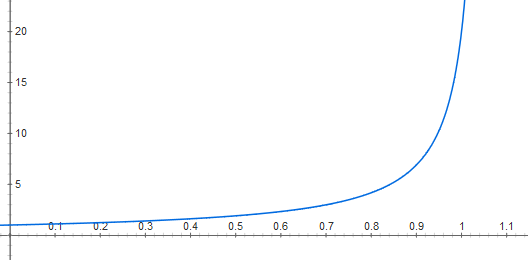
\includegraphics{graph.png}

\item Pour accélérer d'un facteur 2 le code, il faut le vectoriser à 53\%.

\item Pour atteindre une accélération de 10 (moitié de 20) il faut vectoriser le code à 95%.

\item $A=\dfrac{1}{1-0,7+\dfrac{0,7}{20}} \simeq 2,98$. Avec une machine vectorielle deux fois plus puissante : $A=\dfrac{1}{1-0,7+\dfrac{0,7}{40}} \simeq 3,15$. Or il suffirait de vectoriser $\dfrac{20}{19}(1-\dfrac{1}{3,15})=71,8\%$ soit à peine 2\% de code supplémentaire pour obtenir une accélération équivalente.
\end{enumerate}

\end{enumerate}


\paragraph{Ex 2}
\begin{enumerate}
\item
\begin{enumerate}
\item $MIPS = \dfrac{freq}{10^6 . CPI}$. On obtient donc 1,67 MIPS avec le coprocesseur, et 2,78 sans ; ce qui montre bien que les MIPS ne sont pas un bon indicateur de performance.

\item Avec le coprocesseur, on a exécuté $\dfrac{1,08 \cdot 16,67 \cdot 10^6}{10} = 1800360$ instructions, et $\dfrac{13,6\cdot 16.67 \cdot 10^6}{6} = 37785333$ instructions sans.

\item Il y a $1800360-195578 = 1604782$ opérations non flottante par itération, donc l'émulation logicielle a utilisé $37785333-1604782 = 36180551$ instructions pour les opérations flottantes, soit $\dfrac{36180551}{195578} = 185$ instructions entière pour une instruction flottante.
\item On a exécuté 195578 opérations en 1.08 secondes, cela fait donc $\dfrac{195578}{10^6 \cdot 1.08} = 0.181$ MFLOPS.
\end{enumerate}

\item
\begin{enumerate}
\item $MIPS_{base} = \dfrac{nb\_instructions}{10^6 \cdot temps} = \dfrac{I + F\cdot Y}{10^6 \cdot W}$ et $MIPS_{fouet} =  \dfrac{nb\_instructions}{10^6 \cdot temps} = \dfrac{I + F}{10^6 \cdot B}$
\item $I = MPIS_{base}\cdot 10^6 \cdot W - F\cdot Y = 120 \cdot 10^6 \cdot 4 - 50 \cdot 8 \cdot 10^6 = 80\cdot 10 ^6$
\item $B = \dfrac{I+F}{10^6\cdot MIPS_{fouet}} = \dfrac{80\cdot 10^6 + 8\cdot 10 ^6}{10^6 \cdot 80} = 1,1$
\item On exécute $80$ MIPS dont $\dfrac{I}{10^6 \cdot W} = \dfrac{80 \cdot 10 ^6}{10^6 \cdot 4} = 60$ instruction entières, le débit MFLOPS est donc de $20$ MFLOPS avec le coprocesseur.
\item Les MIPS ne signifient rien : le débit MIPS l'utilisant ici est de 80 contre 120 avec, alors que le temps passe de 4 à 1,1. Il faut par contre vérifier que le temps d'exécution est bien moindre sur le programme, i.e. que la perte de MIPS est bien compensée par les opérations flottantes.
\end{enumerate}
\end{enumerate}

\paragraph{Ex 3}
\begin{enumerate}
\item $Acc(scaled)  \leq P + (1-p) \times seq = 8 + (1-8) \times 0.14 = 7.02$
\item On veut conserver un scaled speedup de 7.02. Il faut donc un code à $\dfrac{7.02 - 10}{1-10} = 33,1\%$ parallèle.
\end{enumerate}

\paragraph{Ex 4}
\begin{enumerate}
\item 
\begin{enumerate}
\item
\begin{tabular}{c|c|c|c|c}
& 2 & 3 & 4 & 8\\
\hline
acc & 1,95 & 2,88 & 3,76 & 6,96\\
\hline
eff & 0,977 & 0,963 & 0,94 & 0,869\\
\hline
e & 0,0256 & 0,0208 & 0,0213 & 0,0213\\
\end{tabular}

\item Ce accélérations sont cohérentes : elles sont élevées, ce qui témoigne d'un code fortement parallélisé, mais l'efficacité diminue du fait des synchronisations, des créations de threads et du code non parallélisable. En effet, $e = \dfrac{\frac{1}{acc}-\frac{1}{p}}{1-\frac{1}{p}} = \dfrac{\frac{p \cdot TpsCodeSeq + TpsCodePar}{p\cdot(TpsCodeSeq + TpsCodePar)}-\frac{1}{p}}{1-\frac{1}{p}} = \dfrac{(p-1)\cdot TpsCodeSeq}{(p-1)(TpsCodeSeq + TpsCodePar)} = \dfrac{TpsCodeSeq}{TpsCodeSeq+TpsCodePar}$, e mesure donc la fraction de code séquentiel dans chaque exécution.

\item e $\in [0,1]$ est un indice de la part séquentiel du code : à 0, le code est entièrement parallèle et à 1, il est entièrement  séquentiel. Ici, e$\simeq 0,02$, je dirais donc que le code est donc bien fortement parallélisé.
\end{enumerate}

\item
\begin{enumerate}
\item 
\begin{tabular}{c|c|c|c}
& 2 & 3 & 4\\
\hline
acc & 1,90 & 2,65 & 3,22\\
\hline
eff & 0,95 & 0,88 & 0,81\\
\hline
e & 0,052 & 0,066 & 0,081\\
\end{tabular}

\item Une fois encore, l'efficacité diminue, mais de manière plus franche que pour la question (1). On voit que e augmente, ce qui montre que des synchronisations ont lieu.
\end{enumerate}
\end{enumerate}
\end{document}